 %package list
\documentclass{article}
\usepackage[top=3cm, bottom=3cm, outer=3cm, inner=3cm]{geometry}
\usepackage{multicol}
\UseRawInputEncoding
\usepackage{graphicx}
\usepackage{url}
%\usepackage{cite}
\usepackage{hyperref}
\usepackage{array}
%\usepackage{multicol}
\newcolumntype{x}[1]{>{\centering\arraybackslash\hspace{0pt}}p{#1}}
\usepackage{natbib}
\usepackage{pdfpages}
\usepackage{amsmath}  
\usepackage{multirow}
\usepackage[normalem]{ulem}
\useunder{\uline}{\ul}{}
\usepackage{svg}
\usepackage{xcolor}
\usepackage{listings}
\lstdefinestyle{ascii-tree}{
    literate={├}{|}1 {─}{--}1 {└}{+}1
  }
\lstset{basicstyle=\ttfamily,
  showstringspaces=false,
  commentstyle=\color{red},
  keywordstyle=\color{blue}
}
%\usepackage{booktabs}
\usepackage{caption}
\usepackage{subcaption}
\usepackage{float}
\usepackage{array}

\newcolumntype{M}[1]{>{\centering\arraybackslash}m{#1}}
\newcolumntype{N}{@{}m{0pt}@{}}

%------------------------------ ÍTEMS --------------------------------

\newcommand{\itemEmail}{hchoquehuancaz@unsa.edu.pe}
\newcommand{\itemStudent}{Hernan Andy Choquehuanca Zapana}
\newcommand{\itemCourse}{Fundamentos de la Programacion II}
\newcommand{\itemCourseCode}{1701213}
\newcommand{\itemSemester}{II}
\newcommand{\itemUniversity}{Universidad Nacional de San Agustin de Arequipa}
\newcommand{\itemFaculty}{Facultad de Ingenieria de Produccion y Servicios}
\newcommand{\itemDepartment}{Departamento Academico de Ingenieria de Sistemas e Informatica}
\newcommand{\itemSchool}{Escuela Profesional de Ingenieria de Sistemas}
\newcommand{\itemAcademic}{2023 - B}
\newcommand{\itemInput}{Del 22 Diciembre 2023}
\newcommand{\itemOutput}{Al 23 Diciembre 2023}
\newcommand{\itemPracticeNumber}{03}
\newcommand{\itemTheme}{Herencia en java}

%------------------------------  ------------------------------

\usepackage[english,spanish]{babel}
\usepackage[utf8]{inputenc}
\AtBeginDocument{\selectlanguage{Spanish}}
\renewcommand{\figurename}{Figura}
\renewcommand{\refname}{Referencias}
\renewcommand{\tablename}{Tabla} %esto no funciona cuando se usa babel
\AtBeginDocument{
	\renewcommand\tablename{Tabla}
}

\usepackage{fancyhdr}
\pagestyle{fancy}
\fancyhf{}
\setlength{\headheight}{30pt}
\renewcommand{\headrulewidth}{1pt}
\renewcommand{\footrulewidth}{1pt}
\fancyhead[L]{\raisebox{-0.2\height}{
\includegraphics[width=3cm]{img/logo_episunsa.png}}}
\fancyhead[C]{\fontsize{7}{7}\selectfont	\itemUniversity \\ \itemFaculty \\ \itemDepartment \\ \itemSchool \\ \textbf{\itemCourse}}
\fancyhead[R]{\raisebox{-0.2\height}{
\includegraphics[width=1.2cm]{img/logo_abet}}}
\fancyfoot[L]{Estudiante: Hernan Choquehuanca Zapana}
\fancyfoot[R]{\itemCourse}
\fancyfoot[C]{Página \thepage}

% para el codigo fuente
\usepackage{listings}
\usepackage{color, colortbl}
\definecolor{dkgreen}{rgb}{0,0.6,0}
\definecolor{gray}{rgb}{0.5,0.5,0.5}
\definecolor{mauve}{rgb}{0.58,0,0.82}
\definecolor{codebackground}{rgb}{0.95, 0.95, 0.92}
\definecolor{tablebackground}{rgb}{0.8, 0, 0}

\lstset{frame=tb,
	language=bash,
	aboveskip=3mm,
	belowskip=3mm,
	showstringspaces=false,
	columns=flexible,
	basicstyle={\small\ttfamily},
	numbers=none,
	numberstyle=\tiny\color{gray},
	keywordstyle=\color{blue},
	commentstyle=\color{dkgreen},
	stringstyle=\color{mauve},
	breaklines=true,
	breakatwhitespace=true,
	tabsize=3,
	backgroundcolor= \color{codebackground},
}

%------------------------------ INICIO DEL DOCUMENTO------------------------------

\begin{document}
	
	\vspace*{10px}
	
	\begin{center}	
		\fontsize{17}{17} \textbf{ Informe de Teoría \itemPracticeNumber}
	\end{center}
	\centerline{\textbf{\Large Tema: \itemTheme}}
	%\vspace*{0.5cm}	

	\begin{flushright}
		\begin{tabular}{|M{2.5cm}|N|}
			\hline 
			\rowcolor{tablebackground}
			\color{white} \textbf{Nota}  \\
			\hline 
			     \\[30pt]
			\hline 			
		\end{tabular}
	\end{flushright}	

	\begin{table}[H]
		\begin{tabular}{|x{4.7cm}|x{4.8cm}|x{4.8cm}|}
			\hline 
			\rowcolor{tablebackground}
			\color{white} \textbf{Estudiante} & \color{white}\textbf{Escuela}  & \color{white}\textbf{Asignatura}   \\
			\hline 
			{\itemStudent \par \itemEmail} & \itemSchool & {\itemCourse \par Semestre: \itemSemester \par Código: \itemCourseCode}     \\
			\hline 			
		\end{tabular}
	\end{table}		
	
	\begin{table}[H]
		\begin{tabular}{|x{4.7cm}|x{4.8cm}|x{4.8cm}|}
			\hline 
			\rowcolor{tablebackground}
			\color{white}\textbf{Trabajo} & \color{white}\textbf{Tema}  & \color{white}\textbf{Duración}   \\
			\hline 
			\itemPracticeNumber & \itemTheme & 02 horas   \\
			\hline 
		\end{tabular}
	\end{table}
	
	\begin{table}[H]
		\begin{tabular}{|x{4.7cm}|x{4.8cm}|x{4.8cm}|}
			\hline 
			\rowcolor{tablebackground}
			\color{white}\textbf{Semestre académico} & \color{white}\textbf{Fecha de inicio}  & \color{white}\textbf{Fecha de entrega}   \\
			\hline 
			\itemAcademic & \itemInput &  \itemOutput  \\
			\hline 
		\end{tabular}
	\end{table}


%------------------------------ ACTIVIDADES (TAREA) ------------------------------

\section{Tarea}
	\begin{itemize}		
        \item Ejercicio 01: Crear una clase base denominada Punto que conste de las coordenadas x e y. A partir de esta clase, definir una clase denominada Circulo que tenga las coordenadas del centro y un atributo denominado radio. Entre las funciones miembro de la primera clase, deberá existir una función distancia() que devuelva la distancia entre dos puntos, donde: \newline
        Distancia = ((x2 – x1)2 + (y2 – y1)2)1/2
        Entregable: fase02/trabajo03/Ejercicio1.java
        
        \item Ejercicio 02: Utilizando la clase construida en el ejercicio 01, obtener una clase derivada Cilindro derivada de Circulo. La clase Cilindro deberá tener una función miembro que calcule la superficie de dicho cilindro. La fórmula que calcula la superficie del cilindro es S = 2r(l + r) donde r es el radio del cilindro y l es la longitud.
        Entregable: fase02/trabajo03/Ejercicio2.java

        \item Ejercicio 03: Caso de estudio especial: herencia múltiple. Es un tipo de herencia en la que una clase hereda el estado (estructura) y el comportamiento de más de una clase base. (hay herencia múltiple cuando una clase hereda de más de una clase). Java no permite la herencia múltiple, pero se puede conseguir la implementación de la herencia múltiple usando interfaces. Implemente el siguiente diagrama de clases UML y consiga pruebas válidas.

        \begin{figure}[H]
            \centering
            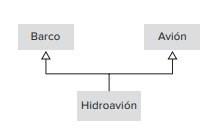
\includegraphics[width=0.31
            \textwidth,keepaspectratio]{img/Ejercicio3.jpg}
        \end{figure}

	\end{itemize}

\newpage

\section{Equipos, materiales y temas utilizados}
	\begin{itemize}
		\item Sistema Operativo Windows 11 Pro 22H2 64 bits.
		\item Vim 9.0.
		\item Git 2.42.0.
		\item Cuenta en GitHub con el correo institucional.
        \item Editor LaTeX en línea Overleaf.
        \item Atributos de clase.
        \item Métodos de clase.
        \item Herencia.
        \item Herencia múltiple.
        \item Clases.
        \item Interfaces.
        
        
	\end{itemize}
	
\section{URL de Repositorio Github}
	\begin{itemize}
		\item URL del Repositorio GitHub para clonar o recuperar.
        \item \url{https://github.com/hernanchoquehuanca/fp2-23b.git}
		\item URL para el trabajo \itemPracticeNumber\ en el Repositorio GitHub.
		\item \url{https://github.com/hernanchoquehuanca/fp2-23b/tree/main/fase02/trabajo03}
	\end{itemize}

\newpage
 
\section{Trabajo \itemPracticeNumber}
        
        
%-----------------------------------------------------------------------------------
%------------------------------------- ACTIVIDADES  --------------------------------
%-----------------------------------------------------------------------------------

% ACTIVIDADESSSS

%\subsection{Actividad 01}

\subsection{Ejercicio 01}


    \begin{itemize}
        \item La clase Punto contiene 2 atributos protegidos, los cuales son las coordenadas del punto creado.
        \item Contiene los setters y getters, además del método distancia el cual se halla con la siguiente fórmula:
    \end{itemize}
    \[
    \text{Distancia} = \sqrt{{(x_2 - x_1)^2 + (y_2 - y_1)^2}}
    \]
    \begin{itemize}
        \item Usando la clase \textcolor{blue}{Math} se implementó el contenido del método distancia().
    \end{itemize}
    \lstinputlisting[language=Java, firstline=17, lastline=40,firstnumber=17,numbers=left]{src/Ejercicio1.java}


    \begin{itemize}
        \item La clase Circulo contiene 2 atributos protegidos que son su radio y el punto de su centro.
        \item Contiene los setters y getters de cada atributo.
    \end{itemize}
    \lstinputlisting[language=Java, firstline=42, lastline=61,firstnumber=42,numbers=left]{src/Ejercicio1.java}

    
    \begin{itemize}
        \item La clase Ejercicio1 contiene el método principal donde se realiza una prueba de las clases anteriormente creadas.
        \item Crea 2 puntos y usando las clases creadas hallamos sus distancias.
    \end{itemize}
    \lstinputlisting[language=Java, firstline=1, lastline=15,firstnumber=1,numbers=left]{src/Ejercicio1.java}


    \begin{itemize}
        \item \textcolor{purple}{PRUEBA DE EJECUCIÓN DEL CÓDIGO (Ejercicio1.java):}
    \end{itemize}
    \begin{figure}[H]
        \centering
        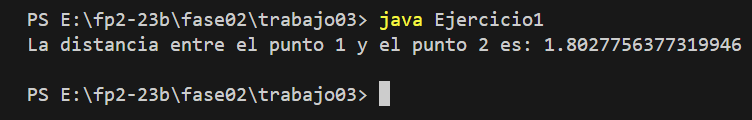
\includegraphics[width=1
        \textwidth,keepaspectratio]{img/Ejercicio1_prueba.png}
    \end{figure}

    \begin{itemize}
        \item Como se vio en el código de la clase Ejercicio1, se crearon 2 puntos (1.0,4.5) y (2.0,6.0).
        \item Entonces al hacer un llamado al método distancia usando estos puntos nos da como resultado lo mostrado.
    \end{itemize}

\newpage
    
\subsection{Ejercicio 02}


    \begin{itemize}
        \item La clase Cilindro hereda de la clase Circulo para de esta forma contener sus atributos y métodos, aparte de ello se implementó el atributo protegido longitud de tipo double.
        \item Contiene sus getters y setters, además también un método que devuelve un double que contiene el valor de la superficie del cilindro usando la siguiente fórmula:
    \end{itemize}
    \[
    \text S = 2r(l + r)
    \]
    \lstinputlisting[language=Java, firstline=16, lastline=30,firstnumber=16,numbers=left]{src/Ejercicio2.java}


    \begin{itemize}
        \item La clase Ejercicio2 contiene el método principal donde se realiza una prueba de la clase Cilindro.
        \item Se crea un Punto llamado centro y luego el Cilindro para hallar su superficie.
    \end{itemize}
    \lstinputlisting[language=Java, firstline=1, lastline=15,firstnumber=1,numbers=left]{src/Ejercicio2.java}


    \begin{itemize}
        \item \textcolor{purple}{PRUEBA DE EJECUCIÓN DEL CÓDIGO (Ejercicio2.java):}
    \end{itemize}
    \begin{figure}[H]
        \centering
        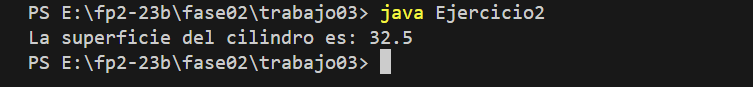
\includegraphics[width=1
        \textwidth,keepaspectratio]{img/Ejercicio2_prueba.png}
    \end{figure}

    \begin{itemize}
        \item Como se vio en el código de la clase Ejercicio2, se creó el Punto centro (3.0,0.0) y (0.0,0.0).
        \item Luego el Cilindro cilindro con su radio y longitud.
        \item Finalmente se hace un llamado para hallar la superficie del cilindro creado y se muestra.
    \end{itemize}

\subsection{Ejercicio 03}
    

    \begin{itemize}
        \item La interfaz Barco contiene métodos propios de una un vehículo que anda en el mar como los que se observa.
    \end{itemize}
    \lstinputlisting[language=Java, firstline=25, lastline=32,firstnumber=25,numbers=left]{src/Ejercicio3.java}
    

    \begin{itemize}
        \item La interfaz Barco contiene métodos propios de una un vehículo que anda en el aire como los que se observa.
    \end{itemize}
    \lstinputlisting[language=Java, firstline=34, lastline=41,firstnumber=34,numbers=left]{src/Ejercicio3.java}
    

    \begin{itemize}
        \item La clase Hidroavion implementa las interfaces Barco y Avion.
        \item Además contiene atributos propios con sus getters y setters.
        \item Sobre-escribe los métodos de ambas interfaces las cuales en su mayoría imprimen en consola y algunos utilizan ciertos atributos.
    \end{itemize}
    \lstinputlisting[language=Java, firstline=43, lastline=145,firstnumber=43,numbers=left]{src/Ejercicio3.java}


    \begin{itemize}
        \item La clase Ejercicio3 contiene el método principal donde se realiza una prueba de la clase Hidroavion.
        \item En este se establecen algunos atributos tales como el modelo y la velocidad.
        \item Finalmente se hace llamado a todos los métodos que contiene la clase.
    \end{itemize}
    \lstinputlisting[language=Java, firstline=1, lastline=23,firstnumber=1,numbers=left]{src/Ejercicio3.java}

    \begin{itemize}
        \item \textcolor{purple}{PRUEBA DE EJECUCIÓN DEL CÓDIGO (Ejercicio2.java):}
    \end{itemize}
    \begin{figure}[H]
        \centering
        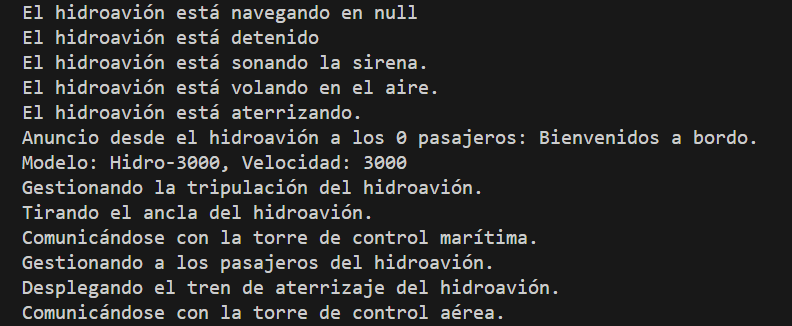
\includegraphics[width=1
        \textwidth,keepaspectratio]{img/Ejercicio3_prueba.png}
    \end{figure}

    \begin{itemize}
        \item Como se vio en el código de la clase Ejercicio3, se creó el Hidroavion con algunos atributos, mas no todos ya se observa en la primera linea que el hidroavion está navegando en null, ya que no fue definido si está en aire o mar.
        \item En cuanto a los demás métodos nos muestran mensajes conforme se implementó en cada método.
    \end{itemize}

%------------------------------ ESTRUCTURA DE LABORATORIO --------------------------

\newpage

\subsection{Estructura de trabajo \itemPracticeNumber} %%CAMBIAR NUMERO DE LAB
\begin{itemize}	
	\item El contenido que se entrega en este trabajo es el siguiente:
\end{itemize}

%---------------------------------------- TREE -------------------------------------

\begin{lstlisting}[style=ascii-tree]

    trabajo03
    |   Ejercicio1.java
    |   Ejercicio2.java
    |   Ejercicio3.java
    |───latex
        |   Informe_Trabajo03.pdf
        |   Informe_Trabajo03.tex
        |───img 
        |       Ejercicio1_prueba.jpg  
        |       Ejercicio2_prueba.jpg  
        |       Ejercicio3_prueba.jpg  
        |       Ejercicio3.jpg  
        |       logo_episunsa.png  
        |       logo_abet.png      
        |       logo_unsa.jpg      
        |───src
            |   Ejercicio1.java
            |   Ejercicio2.java
            |   Ejercicio3.java
            

\end{lstlisting}    

\section{\textcolor{red}{Rúbricas}}
	
\subsection{\textcolor{red}{Entregable Informe}}
	\begin{table}[H]
		\caption{Tipo de Informe}
		\setlength{\tabcolsep}{0.5em} % for the horizontal padding
		{\renewcommand{\arraystretch}{1.5} % for the vertical padding
		\begin{tabular}{|p{3cm}|p{12cm}|}
			\hline
			\multicolumn{2}{|c|}{\textbf{\textcolor{red}{Informe}}}  \\
			\hline 
			\textbf{\textcolor{red}{Latex}} & \textcolor{blue}{El informe está en formato PDF desde Latex,  con un formato limpio (buena presentación) y fácil de leer.}   \\ 
			\hline 
		\end{tabular}
	}
	\end{table}
	
\clearpage

%------------------------------ RÚBRICA DE EVALUACIÓN ------------------------------
 
\subsection{\textcolor{red}{Rúbrica para el contenido del Informe y demostración}}
\begin{itemize}			
	\item El alumno debe marcar o dejar en blanco en celdas de la columna \textbf{Checklist} si cumplió con el ítem correspondiente.
	\item Si un alumno supera la fecha de entrega,  su calificación será sobre la nota mínima aprobada, siempre y cuando cumpla con todos lo ítems.
	\item El alumno debe auto calificarse en la columna \textbf{Estudiante} de acuerdo a la siguiente tabla:
	
    \begin{table}[ht]
    	\caption{Niveles de desempeño}
    	\begin{center}
    		\begin{tabular}{ccccc}
        	\hline
        	& \multicolumn{4}{c}{Nivel}\\
        	\cline{1-5}
        	\textbf{Puntos} & Insatisfactorio 25\%& En Proceso 50\% & Satisfactorio 75\% & Sobresaliente 100\%\\
        	\textbf{2.0}&0.5&1.0&1.5&2.0\\
        	\textbf{4.0}&1.0&2.0&3.0&4.0\\
        	\hline
    		\end{tabular}
    	\end{center}
    \end{table}	
\end{itemize}

%------------------------------------ EVALUACIÓN -----------------------------------

\begin{table}[H]
    \caption{Rúbrica para contenido del Informe y demostración}
    \setlength{\tabcolsep}{0.5em} % for the horizontal padding
    {\renewcommand{\arraystretch}{1.5}% for the vertical padding
    %\begin{center}
    \begin{tabular}{|p{2.7cm}|p{7cm}|x{1.3cm}|p{1.2cm}|p{1.5cm}|p{1.1cm}|}
        \hline
        \multicolumn{2}{|c|}{Contenido y demostración} & Puntos & Checklist & Estudiante & Profesor\\
        \hline
        \textbf{1. GitHub} & Hay enlace URL activo del directorio para el  laboratorio hacia su repositorio GitHub con código fuente terminado y fácil de revisar. &2 &X &2 & \\ 
        \hline
        \textbf{2. Commits} &  Hay capturas de pantalla de los commits más importantes con sus explicaciones detalladas. (El profesor puede preguntar para refrendar calificación). &4 &X &4 & \\ 
        \hline 
        \textbf{3. Código fuente} &  Hay porciones de código fuente importantes con numeración y explicaciones detalladas de sus funciones. &2 &X &2 & \\ 
        \hline 
        \textbf{4. Ejecución} & Se incluyen ejecuciones/pruebas del código fuente  explicadas gradualmente. &2 &X &2 & \\ 
        \hline			
        \textbf{5. Pregunta} & Se responde con completitud a la pregunta formulada en la tarea.  (El profesor puede preguntar para refrendar calificación).  &2 &X &2 & \\ 
        \hline	
        \textbf{6. Fechas} & Las fechas de modificación del código fuente están dentro de los plazos de fecha de entrega establecidos. &2 &X &2 & \\ 
        \hline 
        \textbf{7. Ortografía} & El documento no muestra errores ortográficos. &2 &X &2 & \\ 
        \hline 
        \textbf{8. Madurez} & El Informe muestra de manera general una evolución de la madurez del código fuente,  explicaciones puntuales pero precisas y un acabado impecable.   (El profesor puede preguntar para refrendar calificación).  &4 &X &3 & \\ 
        \hline
        \multicolumn{2}{|c|}{\textbf{Total}} &20 & &19 & \\ 
        \hline
    \end{tabular}
    %\end{center}
    %\label{tab:multicol}
    }
\end{table}
\clearpage

%------------------------------ REFERENCIAS ------------------------------

\section{Referencias}
\begin{itemize}			
    \item \url{https://docs.oracle.com/javase/tutorial/java/javaOO/methods.html}
    \item \url{https://stackoverflow.com/questions/1321122/what-is-an-interface-in-java}
    \item \url{https://es.stackoverflow.com/questions/104165/por-qu%C3%A9-la-herencia-m%C3%BAltiple-no-se-admite-en-java}
\end{itemize}	
	
%\clearpage
%\bibliographystyle{apalike}
%\bibliographystyle{IEEEtranN}
%\bibliography{bibliography}
\end{document}